%Plantilla Memoria Técnica:
%Modificada por: Brenda Mariana Casillas González
%Última Modificación: 02-01-2023

%------------------------------CONFIGURACION DEL DOCUMENTO

\documentclass[12pt,letterpaper,spanish]{report}
\usepackage[table]{xcolor} 
\usepackage[centertags]{amsmath}
\usepackage{amsfonts}
\usepackage{amssymb}
\usepackage{amsthm}
\usepackage[T1]{fontenc}
\usepackage[utf8]{inputenc}
\usepackage{lmodern}
\usepackage[spanish,activeacute]{babel}
% Eliminar o comentar cualquier redefinición de fuentes para evitar conflictos
% \renewcommand{\rmdefault}{lmr}
% \renewcommand{\sfdefault}{lmss}
% \renewcommand{\ttdefault}{lmtt}
\usepackage{epsfig}
\usepackage{booktabs}
\usepackage{graphicx}
\renewcommand{\baselinestretch}{1.5}
\usepackage[numbers]{natbib}
\usepackage[hyphens]{url}
\usepackage{enumerate}
\usepackage{hyperref}

\newenvironment{dedication}{\newpage\large\null\em\vskip1in}%
{\vfill}

\topmargin -1 in \oddsidemargin 0in \evensidemargin 0in
\textwidth 6.5in
\textheight 9in \pagestyle{myheadings}

% -----------------------------------INICIO DEL DOCUMENTO  ---------------------------------------------------------------
\begin{document}


% Para la elaboración de esta memoria técnica se debe usar un editor profesional que soporte Latex, como recomendación se puede usar el WinEdt.

% El resultado que se sube a la plataforma debe ser en formato PDF

% Es importante mencionar que la redacción de este documento se debe hacer en tercera persona, cuidando escrupulosamente la ortografía, redacción y contenido, evitando el uso y abuso de adjetivos.

    
% ----------------------------------- CONTRAPORTADA -------------------------------------------------------------------------
%Se deben modificar los datos de la empresa, proyecto, asesores y alumnos

\thispagestyle{empty}

\begin{table}[ht]
  \centering
    \begin{tabular}{rr}
        \begin{minipage}[b]{0.05\linewidth}
        \hbox{
\psfig{file=LogoUTZMG.jpg,height=1in,width=.8in}}
        \end{minipage}
    &
    \begin{minipage}[b]{.8\linewidth}
        \begin{center}
            \large{UNIVERSIDAD TECNOLÓGICA \\ DE LA ZONA METROPOLITANA DE GUADALAJARA}\\
        \end{center}
    \end{minipage}

    \end{tabular}%
\end{table}%

\begin{center}

\large{\textbf{MEMORIA TÉCNICA REALIZADA EN:}}
 \\  Corporativo Textil JSN, S. de R.L de C.V

%%Logo de la empresa
\centerline{\hbox{
\psfig{file=LogoJASANA.png,height=0.4in,width=1.2in}}}

\large{\textbf{PROYECTO:} Módulo de Gestión de Reprocesos y Reposiciones}

\vspace{0.1in}
\large{\textbf{PARA OBTENER EL GRADO DE:}}

\large{Técnico Superior Universitario (TSU) en:}
\vspace{0.05in}

\large{TECNOLOGÍAS DE LA INFORMACIÓN, ÁREA DESARROLLO DE SOFTWARE MULTIPLATAFORMA }
\\
\large{PRESENTADO POR:}


Victor Manuel Montaño Juanpedro %(Empezando con el nombre  y después apellidos)


Eduardo Isa'ias V'azquez Solís %(Empezando con el nombre  y después apellidos)

\vspace{0.2in}

\begin{tabular}{cc}
    \vspace{0.2in}
    \textbf{ASESOR INDUSTRIAL} & \textbf{ASESOR ACADÉMICO} \\

    Jair Efra'in Barragan Gárcia & Lizbeth Noriega Gútierrez \\
    \multicolumn{2}{c}{\textbf{COORDINADOR DE CARRERA}
    \vspace{0.2in}
    } \\

    \multicolumn{2}{c}{
            Ing. Lizbeth Noriega Gutierrez }
    \end{tabular}

\end{center}
%\vspace{0.1in}
\begin{flushright}\small{ TLAJOMULCO DE ZUÑIGA, JALISCO, AGOSTO DEL 2025} \end{flushright}

\newpage


% ------------------------------  PORTADA -----------------------------------------------------
%Se deben modificar los datos de la empresa, proyecto y alumnos


\thispagestyle{empty}


\begin{center}

 \begin{minipage}[b]{.9\linewidth}
    \begin{center}
        \vspace{0.2in}
        \large{UNIVERSIDAD TECNOLÓGICA DE LA ZONA \\METROPOLITANA DE GUADALAJARA}\\
        \large{DIRECCIÓN DE DESARROLLO Y GESTIÓN DE SOFTWARE}\\
    \end{center}
\end{minipage}
\vspace{0.3in}


\centerline{\hbox{\psfig{file=logoUTZMG.jpg,height=2in,width=1.5in}}}

\LARGE{\textsc{Módulo de Gestión de Reprocesos y Reposiciones}}
% \LARGE{\textbf{Módulo de Gestión de Reprocesos y Reposiciones}} % Alternative: bold only, no small caps

\vspace{0.2in}
\large{\textbf{MEMORIA TÉCNICA REALIZADA EN:}}
 \\  \textsc{Corporativo Textil JSN, S. de R.L de C.V}

\vspace{0.2in}
\large{\textbf{PARA OBTENER EL GRADO DE:}}

\large{Técnico Superior Universitario (TSU) en:}


\large{TECNOLOGÍAS DE LA INFORMACIÓN\\Área, DESARROLLO DE SOFTWARE MULTIPLATAFORMA }
\\

\vspace{0.2in}
\large{PRESENTADO POR:}


\textsc{Víctor Manuel Montaño Juanpedro}  %(Empezando con el nombre  y después apellidos)


\textsc{Eduardo Isaías Vázquez Solís}  %(Empezando con el nombre  y después apellidos)

\vspace{0.2in}
\small{ AGOSTO 2025}
\end{center}
%\vspace{0.1in}


\newpage



% -------------------------------------- DEDICATORIA   ---------------------
% Esta sección es opcional, pero se recomienda que se ponga, se puede redactar hasta el final y tratar que no sea mayor a una cuartilla.

        \thispagestyle{empty}
        \addcontentsline{toc}{chapter}{Agradecimientos}

        \begin{dedication}
           Agradezco a todas las personas .... Agradezco a todas las personas ....
           A Toreto, a mi familia, a mis amigos, a mis profesores, a mi perro, a mi gato, a mi hamster, a mi pez, a mi tortuga y a todos los que me apoyaron en este proyecto.
           Agradezco a mi familia por su apoyo incondicional, a mis amigos por su compañía y motivación, y a mis profesores por su dedicación y enseñanza.
           A la abuelita de caperucita roja por su sabiduría y consejos, a la tortuga por su paciencia y perseverancia, y al lobo por su astucia y determinación.
           Agradezco a todos los que me han apoyado en este proyecto, a los que me han dado su tiempo, su conocimiento y su experiencia.
           Agradezco a Shrek por su amistad y lealtad, a Fiona por su amor y apoyo, y a Burro por su humor y alegría.
           Tambien a mamá coco y a mamá Himelda.


           Y y y y diles que coman tierra
        \end{dedication}


%--------------------------------         ÍNDICE


\tableofcontents


% --------------------------------------- CAPÍTULOS DEL DOCUMENTO  ----------------------------------------
% ____________________________________________________________________________________

\pagenumbering{arabic}
\oddsidemargin 0.2in \textwidth 6.5in \topmargin -0.25in
\textheight 9in \pagestyle{myheadings}

\newpage

% CAPITULO INTRODUCCIÓN. Enmarca y situa el trabajo a realizar. Tiene por objeto proporcionar una visión general del documento.
%____________________________________________________________________________________________________________________


\chapter{Introducción}
\newpage


Esta es la introducción jshdjhsdjkfhsdjk kjsdlkfjskad jdhshdfsdflksk, jdfjsdhjjkdsjkf.
Esta es la introducción jshdjhsdjkfhsdjk kjsdlkfjskad jdhshdfsdflksk, jdfjsdhjjkdsjkf.
Esta es la introducción jshdjhsdjkfhsdjk kjsdlkfjskad jdhshdfsdflksk, jdfjsdhjjkdsjkf.
Esta es la introducción jshdjhsdjkfhsdjk kjsdlkfjskad jdhshdfsdflksk, jdfjsdhjjkdsjkf.
\\




Esta es la introducción jshdjhsdjkfhsdjk kjsdlkfjskad jdhshdfsdflksk, jdfjsdhjjkdsjkf.


% CAPITULO ANTECEDENTES Y DESCIPCIÓN DE LA EMPRESA. Tiene por objeto proporcionar una visión general del documento.
%____________________________________________________________________________________________________________________

\chapter{Antecedentes y Descripción de la Empresa}
\newpage



%Nota: Los puntos que siguen son una propuesta, pongan solo los puntos que apliquen en su empresa y que los permitan poner, también puede agregar otros puntos si lo cree conveniente.

\section{Ubicación}
La empresa Corporativo Textil JSN, S. de R.L de C.V se encuentra ubicada en C. Flaviano Ramos Sur 37, Centro, 45640 Tlajomulco de Zúñiga, Jal. El mapa puede ser consultado en la Figura\ref{a1}

\begin{figure}[htp]
  \centering
  \includegraphics*{mapajasana1.png}
  \caption{Ubicación de la empresa}\label{a1}
\end{figure}



% Poner la dirección y un mapa que puede salir de maps.google.com

\section{Misión}
% Misión proporcionada por la empresa, se debe modificar la redacción a tercera persona.
Proyectar la identidad empresarial de sus clientes a través de la vestimenta de sus colaboradores, considerando su comodidad. Aplica diseños en tendencia, utiliza tecnologías actualizadas y apoya a la fuerza laboral conformada por familias mexicanas.

\section{Visión}
% Visión proporcionada por la empresa, se debe modificar la redacción a tercera persona.
Consolidar una empresa transnacional en la transformación integral de textiles, estandarizando y digitalizando procesos en sus diferentes unidades de negocio para el año 2030.

\section{Organigrama}
% Poner el organigrama proporcionado por la empresa o crear uno en caso de no contar con el.
A continuación en la figura \ref{a2} se presenta el organigrama de la empresa.

\begin{figure}[htp]
  \centering
  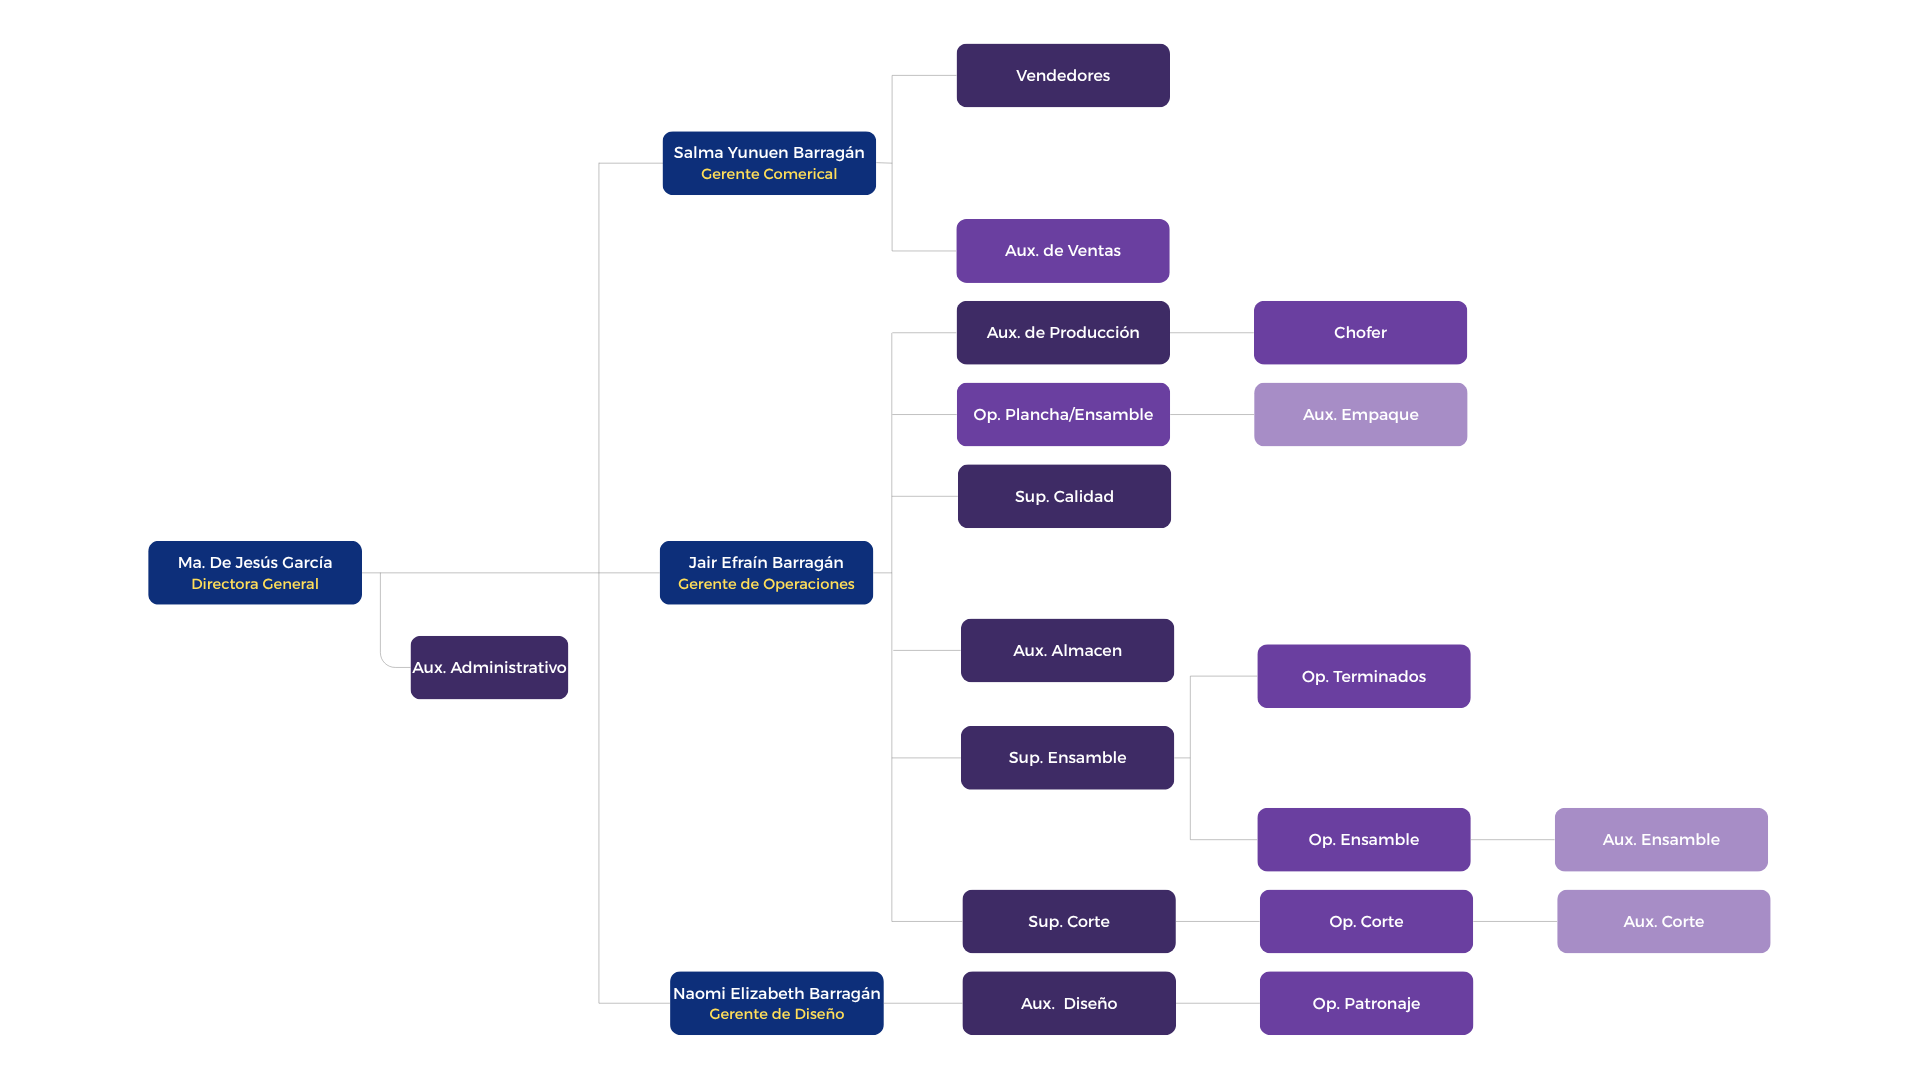
\includegraphics[width=\linewidth]{Organigrama_Jasana3.png}
  \caption{Organigrama de Textil JSN}\label{a2}
\end{figure}

\section{Historia}
En corporativo textil jsn, diseñamos y creamos prendas y textiles para hoteles y empresas de hospitalidad.
Nos dedicamos a que los colaboradores de nuestros clientes estén presentables y cómodos todos los días, priorizando su seguridad e integridad.
Esto lo logramos incorporando tecnologías en nuestras prendas que además aumentan su vida útil.


\newpage

% --------------------------------   CAPITULO PROBLEMÁTICA   --------------------------------------
%____________________________________________________________________________________________________________________



\chapter{Problemática y Descripción del Proyecto}
\newpage

\section{Problemática}

La empresa \textbf{Corporativo Textil JSN}, dedicada a la fabricación de uniformes corporativos, enfrenta actualmente diversas dificultades en el control, trazabilidad y gestión eficiente de los \textit{reprocesos y reposiciones} de piezas defectuosas o dañadas durante la producción. Aunque se utiliza el sistema ERP (Enterprise Resource Planning) Odoo, este proceso específico no se encuentra digitalizado ni debidamente integrado al entorno operativo, generando así múltiples problemáticas en distintas áreas del flujo productivo y administrativo.

Las principales problemáticas detectadas son las siguientes:

\begin{enumerate}
    \item \textbf{Falta de trazabilidad:} No existe un registro digital estandarizado de qué piezas fueron reprocesadas, cuándo, por quién, ni en qué etapa del proceso ocurrieron los daños.
    
    \item \textbf{Procesos manuales:} Actualmente, la información relacionada con daños, responsables y tiempos de corrección se gestiona mediante hojas físicas, lo cual incrementa el riesgo de pérdida de información y errores humanos.
    
    \item \textbf{Descontrol en la gestión por áreas:} Las distintas áreas involucradas en la producción (Diseño, Corte, Ensamble, Planchado, entre otras) operan de forma aislada en cuanto al manejo de reprocesos, sin un sistema común que garantice la continuidad y visibilidad del flujo entre ellas.
    
    \item \textbf{Dificultad para calcular tiempos y costos:} No se cuenta con una herramienta que permita realizar cálculos automáticos del tiempo invertido en cada reproceso, ni estimaciones precisas del costo de materiales e insumos reinvertidos.

\end{enumerate}

Ante este panorama, se vuelve indispensable el desarrollo de un módulo personalizado en Odoo que permita sistematizar la gestión de reprocesos y reposiciones, garantizando control, transparencia, eficiencia operativa, y toma de decisiones basada en información precisa y actualizada.

% En esta sección se deberá redactar un planteamiento de la problemática que se pretende resolver.


%Escribir un resumen de su proyecto en donde se hable del aspecto económico, operativo, técnico, humano, objetivos, etc.
\section{Descripción del Proyecto}

El proyecto se basa en el diseño y desarrollo de un módulo personalizado en Odoo que permita gestionar de forma centralizada, digital y trazable los procesos de reposición y reproceso de piezas defectuosas en la cadena de producción de la empresa Corporativo Textil JSN. El modulo heredará las funcionalidades básicas de Odoo, pero se adaptará específicamente a las necesidades de la empresa para optimizar el flujo de trabajo y mejorar la eficiencia operativa. Tomando como base los módulos de Manofactura y Reparaciones, se implementarán las siguientes características: Lleve el registro de solicitudes de reproceso y reposición, asignación de responsabilidades por área, cálculo automático de tiempos y costos, y generación de reportes históricos.
\subsection*{Aspecto Económico}


\subsection*{Aspecto Operativo}


\subsection*{Aspecto Técnico}


\subsection*{Aspecto Humano}



%Describir cual es el objetivo general que persigue el proyecto.
\subsection{Objetivo General}
\begin{itemize}
\item Desarrollar e implementar un módulo en el ERP Odoo que permita gestionar digitalmente las solicitudes de reproceso y reposición, asegurando trazabilidad, control por área y generación de reportes históricos.
\end{itemize}
%Describir cuales son los objetivos específicos que persigue el proyecto. Mínimo deben ser dos y estos deben abonar al objetivo general
\subsection{Objetivos Específicos}
% \cite{buffett84}
\begin{itemize}
\item Permitir el registro eficiente de solicitudes con folios y datos clave de producción.
\item Asignar y seguir responsabilidades por área en el flujo del reproceso.
\item Automatizar el cálculo de tiempos de reproceso y sus costos estimados.
\item Generar reportes que ayuden en el análisis.
\end{itemize}
%Describir de manera detallada las actividades para el desarrollo de la estadía y/o proyecto (Diagrama de Gantt).
\subsection{Planeación}



%CAPITULO MARCO TEÓRICO: bases teorícas del proyecto. conceptos básicos y antecedentes o información existente.
%____________________________________________________________________________________________________________________

\chapter{Marco Teórico}
\newpage

\section{MongoDB}

Como lo dijo \citeauthor{ArBre}, \citeyear{ArBre}, acelere la innovación a escala, aborde las necesidades de datos de cualquier aplicación rápidamente, acelere el tiempo de obtención de valor y reduzca la complejidad seleccionando y eligiendo lo que necesita de una colección integrada de servicios de infraestructura de datos y bases de datos. Para cumplir con la norma podemos hacer la referencia de esta manera (\citeauthor{mongodb}, \citeyear{mongodb}) y en (\citeauthor{ArBre}, \citeyear{ArBre}).



%CAPITULO DESARROLLO DEL PROYECTO: procedimiento o descripción de las actividades realizadas, como es un desarrollo es importante
%____________________________________________________________________________________________________________________

\chapter{Desarrollo del Proyecto}
\newpage

\section{Requerimientos}

\section{Análisis y Diseño}

\section{Implementación}

\section{Pruebas}


% CAPITULO RESULTADOS(estatus del proyecto y posibles mejoras) Y CONCLUSIONES(problemas presentados, costos, restrasos, cumplimiento de objetivos, etc)
%____________________________________________________________________________________________________________________

\chapter{Resultados y Conclusiones}
\newpage

\section{Resultados}


\section{Conclusiones}


% --------------------------  ANEXOS
%____________________________________________________________________________________________________________________

\newpage

% APENDICE O ANEXO (infoemacion adicional que se quiera anexar o agregar
% BIBLIOGRAFIA
\appendix

%\chapter{Bibliograf\check{}ía}
%\bibliographystyle{apalike}
\bibliographystyle{unsrtnat}

% Eliminar la lista de ítems ficticios para evitar referencias no definidas.


\bibliography{biblio}


\newpage
\chapter{Glosario}

\begin{description}
  \item[Asesor Académico] Persona encargada de regañar a los alumnos
\end{description}

\begin{description}
  \item[ERP(Enterprise Resource Planning)]  Sistema integrado que permite coordinar y 
  optimizar procesos empresariales clave, como finanzas, recursos humanos, logística y producción. 
  Se trata de mucho más que una herramienta tecnológica, ya que busca alinear distintas funciones organizacionales a través de una sola plataforma 
  (O'Brien y Marakas, 2010, como se citó en Hammouch, 2024). %se debe referenciar
  %añadir esto como referencia en la bibliografía:
  % Hammouch,   H.   (2024).   Enhancing   Management   Control   Through   ERP   Systems:   A Comprehensive Literature Review.IRASD Journal of Management,6(3), 125–133.https://doi.org/10.52131/jom.2024
\end{description}
%Otro apendice



\end{document}